\documentclass[10pt]{beamer}
\usetheme{Madrid}
\usecolortheme{seahorse}
\usepackage{amsmath,amssymb,bm}
\usepackage{tikz}
\usetikzlibrary{arrows.meta,positioning}
\setbeamertemplate{navigation symbols}{}

\begin{document}

% =====================================================================
\begin{frame}{Normalizing flow $f_0$ in one slide}
\small
\textbf{Idea:} model the unknown initial DF $f_0(z_0,w_0)$ as a
\emph{simple source density deformed by a trainable bijection}.

\vspace{2pt}
\begin{itemize}\setlength\itemsep{2pt}
\item \textbf{Source density:} 2-D standard Gaussian,
      $\bm u \sim \mathcal N(\bm 0, I)$,
      $\;p_{\rm base}(\bm u)=\tfrac{1}{2\pi}e^{-\|\bm u\|^2/2}$.
\item \textbf{Bijection:} stack of $K$ RealNVP \emph{affine coupling layers} ---
      keep one coordinate, affinely move the other, with scale/shift a small
      neural net of the kept one (roles alternate layer to layer):
      \[
      (a,\,b)\;\longmapsto\;\Bigl(a,\;\bigl(b-t(a)\bigr)\,e^{-s(a)}\Bigr),
      \qquad s,t = \mathrm{MLP}(a).
      \]
      Invertible in closed form: $a$ is untouched, so $s(a),t(a)$ are
      recomputable --- the MLP is never inverted.
\item \textbf{Jacobian is free:} triangular $\Rightarrow$
      $\log\lvert\det J_k\rvert = -s_k(a)$; over the stack they add.
\item \textbf{Density} (change of variables, physical units):
      $\;\log f_0^{\rm flow}(z_0,w_0)=
      -\tfrac12\|\bm u\|^2-\log 2\pi
      +\sum_{k}(-s_k)-\log(\sigma_z\sigma_w)$.
\end{itemize}

\vspace{4pt}
\centering
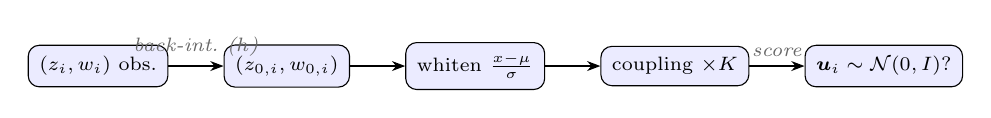
\begin{tikzpicture}[node distance=7mm, every node/.style={font=\scriptsize},
    box/.style={draw, rounded corners, fill=blue!8, inner sep=4pt},
    lbl/.style={font=\scriptsize\itshape, text=black!60}]
\node[box] (obs)  {$(z_i,w_i)$ obs.};
\node[box, right=of obs]  (back) {$(z_{0,i},w_{0,i})$};
\node[box, right=of back] (std)  {whiten $\frac{x-\mu}{\sigma}$};
\node[box, right=of std]  (cpl)  {coupling $\times K$};
\node[box, right=of cpl]  (base) {$\bm u_i \sim \mathcal N(0,I)$?};
\draw[-{Stealth}] (obs)  -- node[above,lbl]{back-int.\ ($h$)} (back);
\draw[-{Stealth}] (back) -- (std);
\draw[-{Stealth}] (std)  -- (cpl);
\draw[-{Stealth}] (cpl)  -- node[above,lbl]{score} (base);
\end{tikzpicture}

\end{frame}

% =====================================================================
\begin{frame}{Static Gaussian vs.\ normalizing flow: the likelihoods}
\small
Both back-integrate each star through the trial potential,
$(z_i,w_i)\xrightarrow{h}(z_{0,i},w_{0,i})$, and use Liouville
($f_{\rm obs}=f_0$ along orbits; symplectic $\Rightarrow$ no Jacobian).
\textbf{Only the role of $f_0$ differs.}

\vspace{4pt}
\begin{columns}[T]
\begin{column}{0.48\textwidth}
\centering \textbf{Static Gaussian $f_0$}
\[
\ln\mathcal L(h)=
-\sum_i\left[\frac{z_{0,i}(h)^2}{2\bar\sigma_z^2}
            +\frac{w_{0,i}(h)^2}{2\bar\sigma_w^2}\right]+\mathrm{c},
\]
\vspace{-4pt}
\[
\max_{\,h\ \text{only}}\ \ln\mathcal L(h)
\]
\begin{itemize}\scriptsize\setlength\itemsep{1pt}
\item $\bar\sigma_z,\bar\sigma_w$ \textbf{frozen} (possibly wrong).
\item Fixed target shape $\Rightarrow$ $h$ absorbs any $f_0$ mismatch
      $\Rightarrow$ \textbf{bias}, but sharp ($\pm1$\,pc, init-independent).
\end{itemize}
\end{column}
\hfill
\begin{column}{0.48\textwidth}
\centering \textbf{Flow $f_0$ (Test 9/10)}
\[
\ln\mathcal L(h,\theta)=\sum_{i}\ln
f_{\theta}\Bigl(z_{0,i}(h),\,w_{0,i}(h)\Bigr),
\]
\vspace{-4pt}
\[
\max_{\,h,\ \theta\ \text{\textbf{jointly}}}\ \ln\mathcal L(h,\theta)
\]
\begin{itemize}\scriptsize\setlength\itemsep{1pt}
\item $\theta$ = coupling nets: target \textbf{reshapes itself} to the
      cloud of the current $h$ $\Rightarrow$ no mismatch to absorb
      $\Rightarrow$ \textbf{no parametric bias}.
\item But $f_\theta$ can fit the cloud of \emph{any} $h$ $\Rightarrow$
      likelihood flattens; $h$ pinned only by \emph{finite capacity}
      (flow can't fit wound-up spirals of wrong $h$).
\end{itemize}
\end{column}
\end{columns}

\vspace{4pt}
\centering
\colorbox{blue!10}{\parbox{0.94\textwidth}{\centering\scriptsize
Same data, physics, estimator --- one line changes:
$\mathcal N_{\bar\sigma}\to f_\theta$, with $\theta$ joining the fit.\quad
Rigid $f_0$: sharp but biased.\; Flow $f_0$: unbiased but only
capacity-constrained.}}

\end{frame}

\end{document}
